\documentclass[11pt,a4paper]{article}

\usepackage[T1]{fontenc}
\usepackage[utf8]{inputenc}
\usepackage{newtxtext,newtxmath}
\usepackage[margin=1in,headheight=15pt]{geometry}
\usepackage{microtype}
\usepackage{setspace}
\setstretch{1.08}

\usepackage{amsmath,mathtools,bm}
\usepackage{booktabs,tabularx,threeparttable,array}
\usepackage{graphicx,caption,float}
\usepackage{enumitem}
\usepackage{xcolor}
\usepackage{fancyhdr}
\usepackage{titlesec}
\usepackage{natbib}
\usepackage{hyperref}
\usepackage[nameinlink,noabbrev]{cleveref}

\definecolor{ink}{HTML}{17212B}
\definecolor{accent}{HTML}{8A3D32}
\definecolor{accentlight}{HTML}{F7EFED}
\definecolor{rulegray}{HTML}{D6DCE1}
\definecolor{evidenceblue}{HTML}{1F5A75}

\hypersetup{
  colorlinks=true,
  linkcolor=accent,
  citecolor=accent,
  urlcolor=accent,
  pdftitle={When Volatility Is Not a Sufficient State},
  pdfauthor={Yitian Chen}
}

\titleformat{\section}
  {\Large\bfseries\color{ink}}
  {\thesection}{0.65em}{}
  [\vspace{0.2em}\color{accent}\titlerule]
\titleformat{\subsection}
  {\large\bfseries\color{ink}}
  {\thesubsection}{0.55em}{}

\setlist[itemize]{leftmargin=1.35em,itemsep=0.25em,topsep=0.35em}
\setlist[enumerate]{leftmargin=1.6em,itemsep=0.25em,topsep=0.35em}
\captionsetup{font=small,labelfont=bf,labelsep=period}
\setlength{\parindent}{1.25em}
\setlength{\parskip}{0.12em}
\setlength{\tabcolsep}{5pt}
\renewcommand{\arraystretch}{1.12}
\graphicspath{{figures/}}

\pagestyle{fancy}
\fancyhf{}
\fancyhead[L]{\small\color{ink}Volatility-state transportability}
\fancyhead[R]{\small\color{ink}Exploratory replication}
\fancyfoot[C]{\thepage}
\renewcommand{\headrulewidth}{0.35pt}
\renewcommand{\headrule}{\hbox to\headwidth{\color{rulegray}\leaders\hrule height \headrulewidth\hfill}}

\newenvironment{evidencebox}
  {\begin{center}\begin{minipage}{0.94\linewidth}\color{evidenceblue}\small
   \hrule\vspace{0.5em}}
  {\vspace{0.5em}\hrule\end{minipage}\end{center}}

\newcolumntype{Y}{>{\raggedright\arraybackslash}X}


\title{When Volatility Is Not a Sufficient State:\\
\large A Cross-Market Replication in Chinese Futures}
\author{Yitian Chen\\
\small Independent Research Project}
\date{Exploratory replication draft -- July 2026}

\begin{document}

\maketitle
\thispagestyle{empty}

\begin{abstract}
We conduct a methodology-locked cross-market replication of the volatility-based
momentum--reversal switching rule proposed for equities by \citet{butt2023}. The setting
is a broad cross-section of Chinese commodity and financial futures. The mapping uses
causal main-contract selection, same-contract returns, an 11-month momentum signal that
skips the most recent month, a one-month reversal signal, and a five-year rolling
volatility distribution. The strategy holds momentum unless lagged market volatility is
in its highest quartile, in which case it holds reversal. After the state-history
requirement, 66 monthly observations are evaluable. Under a lagged open-interest-notional
market proxy, the switch has a higher endpoint than momentum, but its mean monthly
increment is economically small and statistically indistinguishable from zero. Reversal
beats momentum in only 4 of 14 high-volatility months, and one event determines the sign
of the average advantage. Under an equal-product market proxy, high-volatility momentum
outperforms reversal and the switch underperforms momentum. The volatility proxies are
correlated, yet their quartile assignments agree in only 42.4\% of holding months.
High-volatility months exhibit higher cross-product correlation, dispersion, and
directional coherence, showing that volatility captures shock intensity. It does not,
however, uniquely identify shock direction, source, breadth, or stage. The evidence
therefore rejects a transportable volatility-only router in this sample without rejecting
momentum, reversal, or state-dependent allocation more generally.

\end{abstract}

\vspace{0.7em}
\noindent\textbf{Keywords:} Chinese futures; cross-sectional momentum;
short-term reversal; volatility states; cross-market replication; model transportability.

\vspace{0.4em}
\noindent\textbf{JEL classification:} C22, C58, G11, G12, G17.

\vfill
\begin{evidencebox}
\textbf{Evidence status.} This manuscript reports a methodology-locked but exploratory
cross-market replication. The evaluable period contains 66 monthly observations after
the five-year state-history requirement. No threshold, market proxy, sleeve, sector, or
universe was selected using the reported returns. The results do not establish a trading
rule and have no untouched confirmatory period.
\end{evidencebox}

\clearpage
\section{Introduction}

Cross-market replication is most informative when it tests not only whether a return
pattern survives, but whether the state variable retains the economic meaning assigned
to it in the source market. This distinction matters for volatility-based strategy
selection. In equities, high market volatility often co-occurs with market distress,
funding constraints, liquidity demand, and subsequent rebound states in which momentum
can crash and recent losers can reverse. A scalar volatility measure can therefore act
as a compact proxy for a richer joint state.

\citet{butt2023} use this idea to propose a constant-leverage switching rule. The rule
holds cross-sectional momentum when current market volatility lies in the first three
quartiles of its trailing five-year distribution and holds short-term reversal in the
highest quartile. Its appeal is practical as well as economic: it avoids the ex-post
leverage normalization used by some volatility-scaled momentum strategies and can be
specified before next-month returns are observed.

We ask whether that same state variable is sufficient in Chinese futures. Futures are a
demanding transportability test. Their cross-section spans financial contracts,
industrial inputs, agricultural commodities, energy, and other products whose price
changes originate in different cash-market constraints. They also lack a unique analogue
of the equity market-capitalization portfolio. A high aggregate volatility observation
may reflect a broad deleveraging episode, a sector-specific supply shock, a policy change,
or several unrelated shocks occurring simultaneously. These states need not imply the
same next-month ranking of momentum and reversal.

The empirical design is deliberately restrictive. We translate the published rule before
viewing the replication returns; retain the fixed 75th-percentile boundary; use all
eligible products rather than an outcome-selected subset; and report two defensible
futures-market return proxies separately. We do not search for a better percentile after
observing the results. This converts proxy sensitivity and event concentration into
falsification evidence rather than tuning opportunities.

The results do not support a robust replication. The primary switch earns a gross
arithmetic annual return of 13.69\%, compared with 13.25\% for momentum, but the
increment has a HAC $t$-statistic of only 0.06. Reversal beats momentum in 4 of 14
primary-proxy high-volatility months. The mean advantage is positive only because of one
large event; the median and the mean excluding that event are negative. More importantly,
an equal-product volatility proxy reverses the Q4 sleeve ranking and produces a router
that underperforms momentum. The two volatility series have a correlation of 0.83, yet
their quartile states agree in only 42.4\% of strategy months.

The negative result is not equivalent to saying that volatility is noise. In the primary
proxy, Q4 signal months have the highest average pairwise product correlation,
cross-sectional dispersion, and directional coherence. Volatility successfully measures
the intensity and commonality of shocks. What it fails to identify is whether the shock
is trend-generating or reversal-generating.

The paper makes four contributions. First, it provides a transparent cross-asset
replication of a fixed equity routing rule in a heterogeneous futures market. Second, it
shows why high correlation between alternative state measures is not enough when the
decision depends on crossing a quantile boundary. Third, it separates an event-level
crash-hedge echo from a stable conditional relation. Fourth, it develops an economic
interpretation of state insufficiency: volatility is an intensity scalar, whereas
strategy selection requires information about direction, source, breadth, and shock
stage.

\section{Literature and Economic Mechanism}

\subsection{Momentum, crashes, and volatility}

Cross-sectional momentum buys past winners and sells past losers
\citep{jegadeesh1993}. Its long-run average profitability coexists with severe episodic
losses. \citet{daniel2016} show that momentum crashes are predictable in panic states
and are associated with market rebounds and time-varying exposure. Volatility management
can reduce such losses, although scaling changes leverage and requires a target-risk
choice \citep{barroso2015}.

\citet{butt2023} replace continuous scaling with discrete strategy selection. Their
switch is motivated by two conditional relations: high market volatility predicts weaker
momentum and stronger short-term reversal. The source paper interprets reversal partly as
compensation for supplying liquidity when demand for immediacy is high. This view is
consistent with evidence that short-horizon return reversals become stronger when market
liquidity is scarce \citep{nagel2012,jegadeesh1990,lehmann1990}.

The source mechanism is therefore richer than the statement ``high volatility causes
reversal.'' Volatility proxies for a joint state containing distress, prior losses,
funding pressure, liquidity demand, changing winner--loser betas, and a possible market
rebound. The router works only if that joint state is sufficiently stable across time and
markets.

\subsection{Why futures are a useful external test}

Futures markets contain well-documented momentum-related phenomena, including time-series
momentum \citep{moskowitz2012} and momentum combined with term-structure information in
commodity allocation \citep{fuertes2010}. These results do not imply that an equity
cross-sectional state variable transfers mechanically. Futures prices respond directly
to inventories, storage economics, production constraints, hedging demand, interest
rates, currencies, and policy. A shock can represent slow information incorporation and
trend continuation rather than temporary liquidity pressure.

This difference suggests a transportability hypothesis. In equities, a market-level
volatility scalar may summarize a relatively coherent distress state. In a broad futures
cross-section, the same scalar may aggregate economically distinct shocks. The proper
test is therefore not only whether the primary router has a higher sample return, but
whether the conditional sleeve ranking is monotonic, representative across high-volatility
months, and stable to a reasonable definition of the futures ``market.''

\section{Cross-Market Mapping and Hypotheses}

\subsection{The unavoidable mapping problem}

An equity index has a natural market-capitalization weighting. Futures open interest is
not corporate ownership, and the number of outstanding contracts cannot be compared
across products without accounting for price units and multipliers. We therefore use two
market-return proxies that are defensible for different reasons.

The primary proxy weights each available product return by lagged open-interest notional:
\begin{equation}
  w^{OI}_{i,d}=
  \frac{P_{i,d-1}M_iOI_{i,d-1}}
  {\sum_j P_{j,d-1}M_jOI_{j,d-1}},
  \qquad
  r^{M,OI}_{d}=\sum_i w^{OI}_{i,d}r_{i,d},
  \label{eq:oi-market}
\end{equation}
where $P$, $M$, and $OI$ denote lagged price, contract multiplier, and lagged open
interest. This proxy emphasizes products with larger outstanding notional activity. The
robustness proxy assigns equal weight to each available product return. It emphasizes the
typical product rather than the concentration of notional activity.

Neither proxy is declared universally correct. Their disagreement is part of the test.
Choosing the proxy that produces the best endpoint after observing returns would replace
cross-market replication with specification search.

\subsection{Pre-specified hypotheses}

The source mechanism implies three directional hypotheses:

\begin{enumerate}
  \item Momentum should dominate reversal in volatility states Q1--Q3.
  \item Reversal should strengthen and dominate momentum in Q4.
  \item The Q4 switch should improve momentum, reversal, and a static equal blend without
  depending on one event or one market proxy.
\end{enumerate}

The third condition is stricter than comparing the router only with reversal. A selector
can appear successful simply because it spends most months in the stronger sleeve. It
must add information relative to the best standalone sleeve and to a no-state
diversification benchmark.

\subsection{Why the static benchmark is 50/50}

Momentum and reversal are constructed with the same unit long and unit short gross
exposure. Their static blend is
\begin{equation}
  R^{50/50}_{m}=0.5R^{MOM}_{m}+0.5R^{REV}_{m}.
\end{equation}
The equal allocation is not estimated. It is the parameter-free question: does dynamic
state selection improve on holding both sleeves without forecasting the state? It is not
claimed to be the optimal ex-post combination.

\section{Data and Empirical Design}

\subsection{Sample construction}

The daily panel spans January 2016 through June 2026 and begins from 88 futures products
across 13 broad economic sectors. Daily main contracts are selected causally using only
lagged activity. Returns are computed only when consecutive product observations refer to
the same underlying contract, preventing a change in quoted delivery contract from being
treated as an asset return. The analysis does not delete products or sectors because of
realized strategy performance.

\begin{table}[H]
\centering
\caption{Sanitized sample and design summary}
\label{tab:sample}
\begin{tabular}{lr}
\toprule
Item & Value \\
\midrule
Daily data span & 2016-01 to 2026-06 \\
Initial product set & 88 \\
Broad sectors & 13 \\
Evaluation period & 2021-01 to 2026-06 \\
Evaluation months & 66 \\
Mean eligible products per month & 65.9 \\
Momentum formation / skip & 11 months / 1 month \\
Reversal formation & 1 month \\
Long and short tails & 10\% each \\
Volatility history & 60 months \\
Router boundary & Fixed Q4 \\
\bottomrule
\end{tabular}
\end{table}

The distinction between the full data span and the strategy evaluation span is
important. Five years of observations are required before a monthly volatility can be
placed in its trailing distribution. The approximately ten-year panel therefore yields
only 66 evaluable holding months and 14 primary-proxy Q4 months. The effective tail-state
sample is small even though the underlying daily panel is broad.

\subsection{Sleeves}

For holding month $m$, the momentum score compounds product returns from $m-12$ through
$m-2$:
\begin{equation}
  MOM_{i,m}=\prod_{k=2}^{12}(1+R_{i,m-k})-1.
\end{equation}
The momentum sleeve buys the top decile and sells the bottom decile. The reversal score
is the most recent complete-month return,
\begin{equation}
  REVScore_{i,m}=R_{i,m-1},
\end{equation}
and the portfolio buys prior losers and sells prior winners. Each long and short leg is
equally weighted and has unit gross exposure.

\subsection{Volatility states and causal routing}

For each proxy, monthly market volatility is the sample standard deviation of daily
market returns within month $t$:
\begin{equation}
  \sigma_t=sd\{r^M_d:d\in t\}.
\end{equation}
The current observation is ranked in the trailing 60-month volatility distribution. The
state determined in $t$ first affects holdings in $t+1$:
\begin{equation}
R^{Router}_{t+1}=
\begin{cases}
R^{REV}_{t+1}, & \sigma_t\in Q4,\\
R^{MOM}_{t+1}, & \sigma_t\in\{Q1,Q2,Q3\}.
\end{cases}
\label{eq:router}
\end{equation}
The 75th-percentile boundary and both market proxies were specified without searching the
reported return sample.

\subsection{Evaluation logic}

We report arithmetic annual return, annualized volatility, Sharpe ratio, maximum
drawdown, conditional monthly means, and heteroskedasticity-and-autocorrelation-consistent
tests of return differences. Robust replication additionally requires that the Q4
relation be positive and representative across months, survive the equal-product proxy,
and improve on momentum and the static blend. Indicative implementation adjustments are
treated as a secondary feasibility check rather than a reason to modify signals.

\section{Replication Results}

\subsection{Standalone sleeve economics}

\begin{table}[H]
\centering
\caption{Gross strategy performance}
\label{tab:performance}
\begin{tabular}{lrrr}
\toprule
Strategy & Annual return & Sharpe & Maximum drawdown \\
\midrule
Momentum & 13.25\% & 0.46 & $-39.35\%$ \\
Reversal & $-2.89\%$ & $-0.10$ & $-50.48\%$ \\
Static 50/50 & 5.18\% & 0.33 & $-17.61\%$ \\
Primary router & 13.69\% & 0.51 & $-36.24\%$ \\
Equal-proxy router & 7.77\% & 0.30 & $-47.37\%$ \\
\bottomrule
\end{tabular}
\end{table}

Momentum is positive in the evaluation sample, although its risk-adjusted performance is
modest and its drawdown is large. Reversal has negative unconditional economics. This is
already a challenge for the source mechanism: a router can create stable value only if
the replacement sleeve is economically useful in the states in which it is selected.

The primary router has the highest endpoint and a slightly smaller drawdown than
momentum. It does not dominate the static blend on drawdown, and the equal-proxy router
performs materially worse than momentum. \Cref{fig:performance} illustrates why endpoint
ranking alone is an incomplete replication criterion.

\begin{figure}[H]
\centering
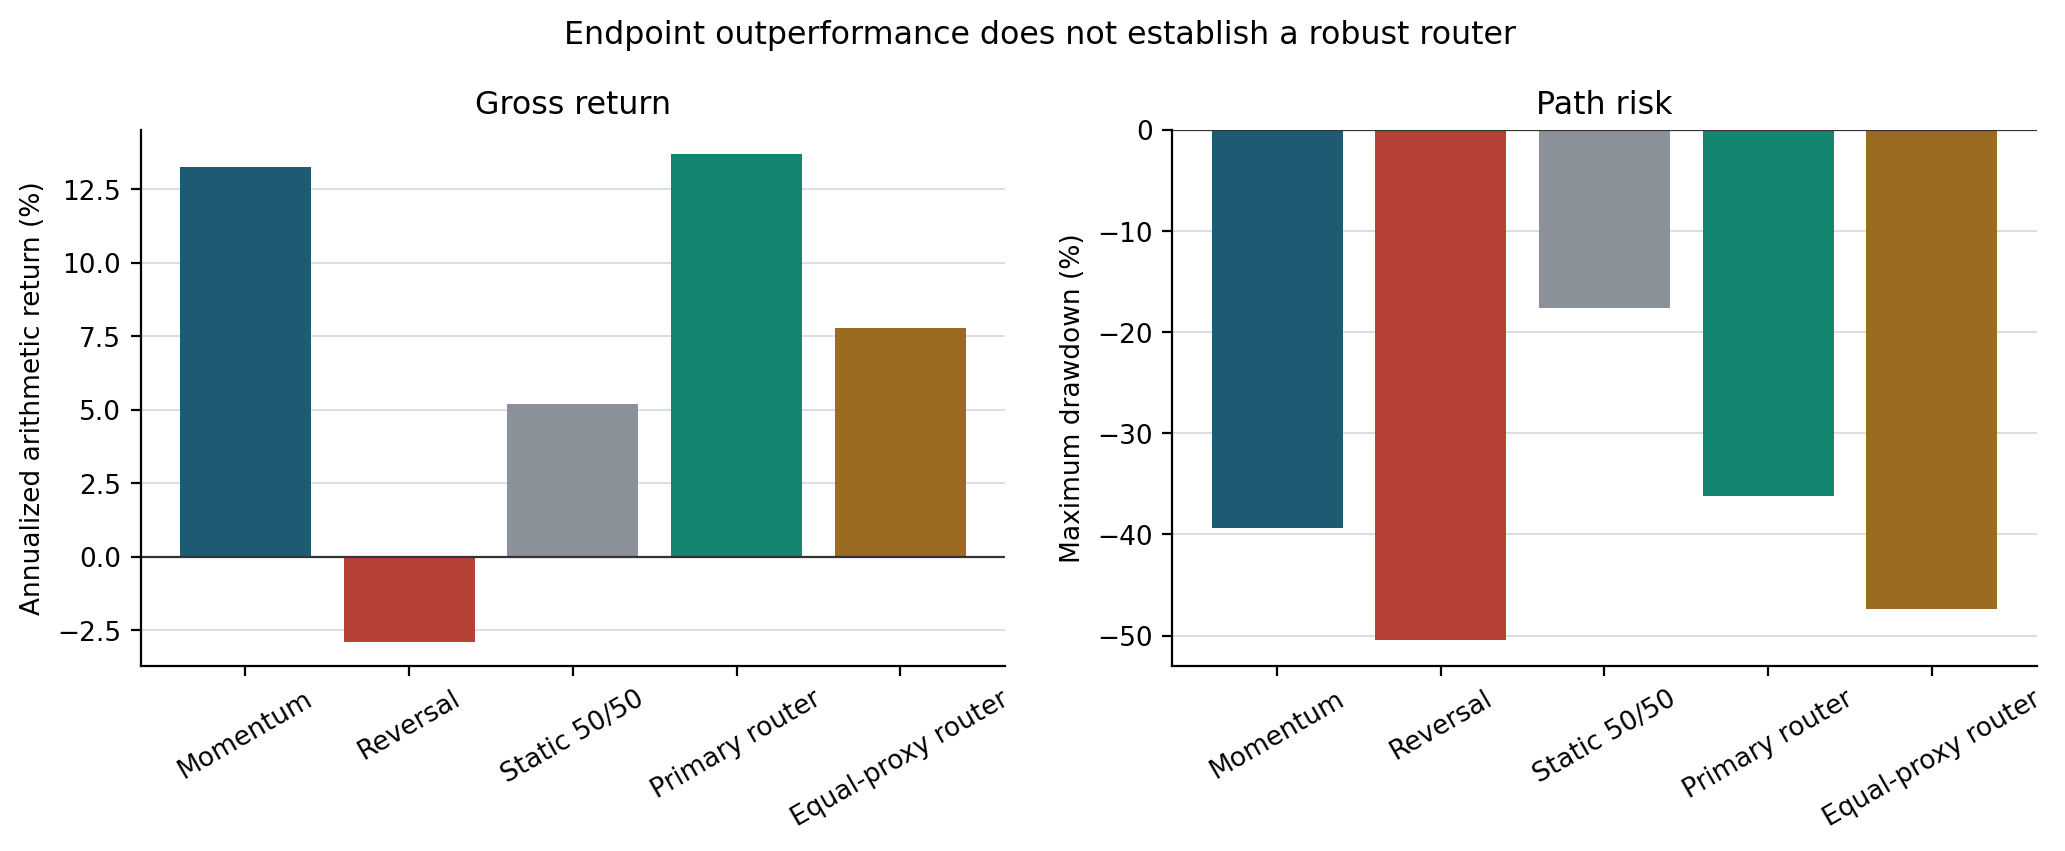
\includegraphics[width=0.96\textwidth]{fig01_public_performance.png}
\caption{Gross performance and path risk. The two routers differ only in the definition
of aggregate market volatility.}
\label{fig:performance}
\end{figure}

\subsection{The conditional relation is neither monotonic nor proxy-stable}

Under the primary proxy, reversal exceeds momentum in Q2 and Q4, while momentum strongly
dominates in Q3. In Q4 both sleeves lose money: momentum averages $-0.71\%$ per month and
reversal averages $-0.54\%$. The 17 basis-point difference satisfies the source
direction only weakly and does not show that reversal becomes a positive high-volatility
sleeve.

Under equal-product volatility, the Q4 ranking reverses. Momentum averages 2.40\% per
month and reversal 0.90\%. Q3, not Q4, is the state in which reversal exceeds momentum.
The conditional pattern is therefore not a monotonic function of volatility and is not
stable to a reasonable market definition.

\begin{figure}[H]
\centering
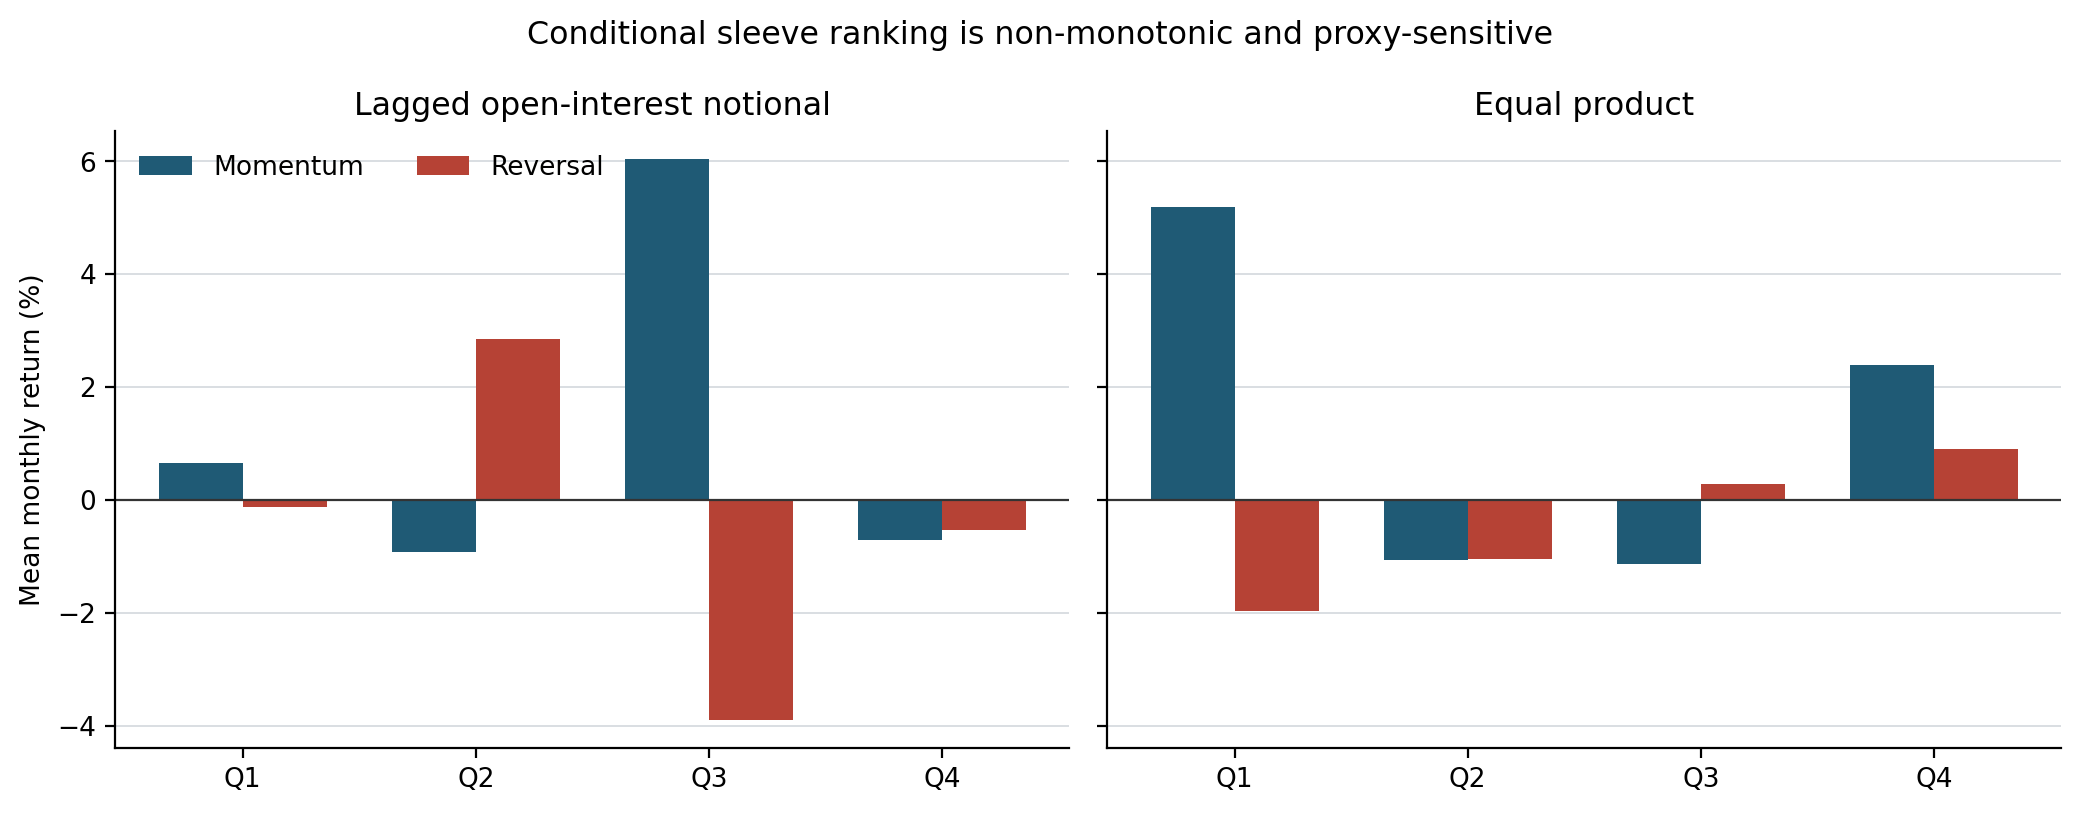
\includegraphics[width=0.96\textwidth]{fig02_public_conditional_returns.png}
\caption{Conditional gross returns by the lagged volatility state used for the holding
month.}
\label{fig:conditional}
\end{figure}

\subsection{The primary improvement is event-concentrated}

The primary router improves on momentum by only 3.69 basis points per month on average,
with a HAC $t$-statistic of 0.06. Among 14 Q4 months, reversal wins four. Its mean
advantage over momentum is 0.17\% per month, but the median is $-2.68\%$. One event has a
34.28 percentage-point reversal advantage; excluding it, the mean Q4 advantage is
$-2.45\%$ per month.

\begin{figure}[H]
\centering
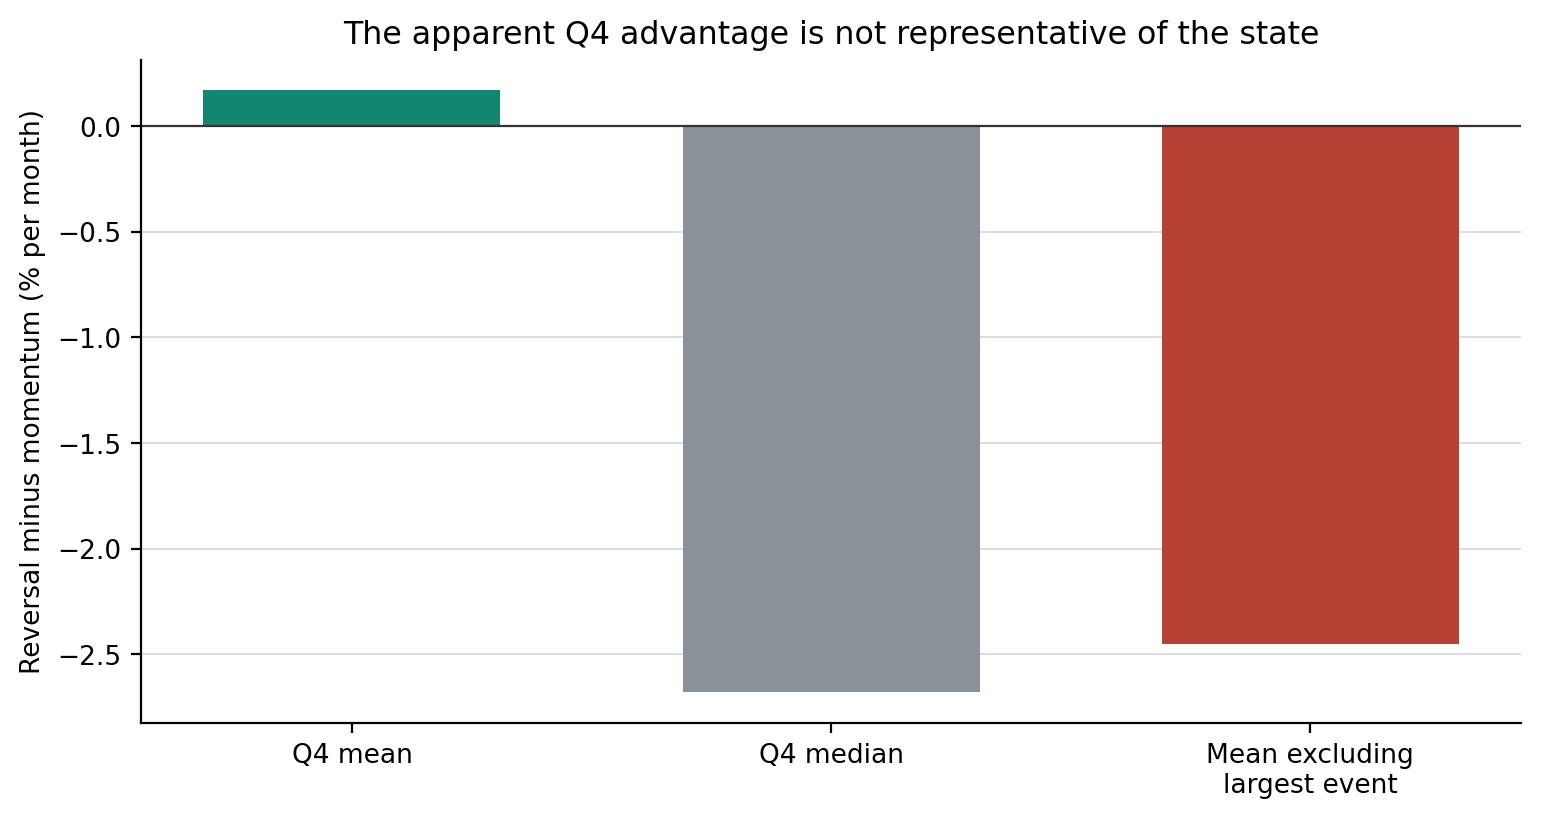
\includegraphics[width=0.78\textwidth]{fig05_public_event_influence.png}
\caption{Aggregate Q4 influence diagnostics. The event date and return series are not
included in the sanitized evidence package.}
\label{fig:influence}
\end{figure}

This pattern is better described as an event-level momentum-crash hedge echo than a
stable Q4 routing relation. A single successful rescue is economically interesting, but
it does not make high volatility a sufficient switching condition.

\section{Why Volatility Is Not a Sufficient State}

\subsection{Proxy correlation is not decision stability}

The two monthly volatility series have a correlation of 0.83. If volatility were used as
a continuous descriptive variable, this might appear reassuring. The router, however,
uses a discontinuous decision: crossing the rolling 75th percentile changes the entire
portfolio from momentum to reversal. Small differences in weighting or rank near the
boundary can therefore produce different holdings.

Across the 66 holding months, the two proxies assign the same quartile only 42.4\% of the
time. Their Q4 sets have a Jaccard overlap of 54.5\%. \Cref{fig:stability} distinguishes
correlation in levels from agreement in the actual decision state.

\begin{figure}[H]
\centering
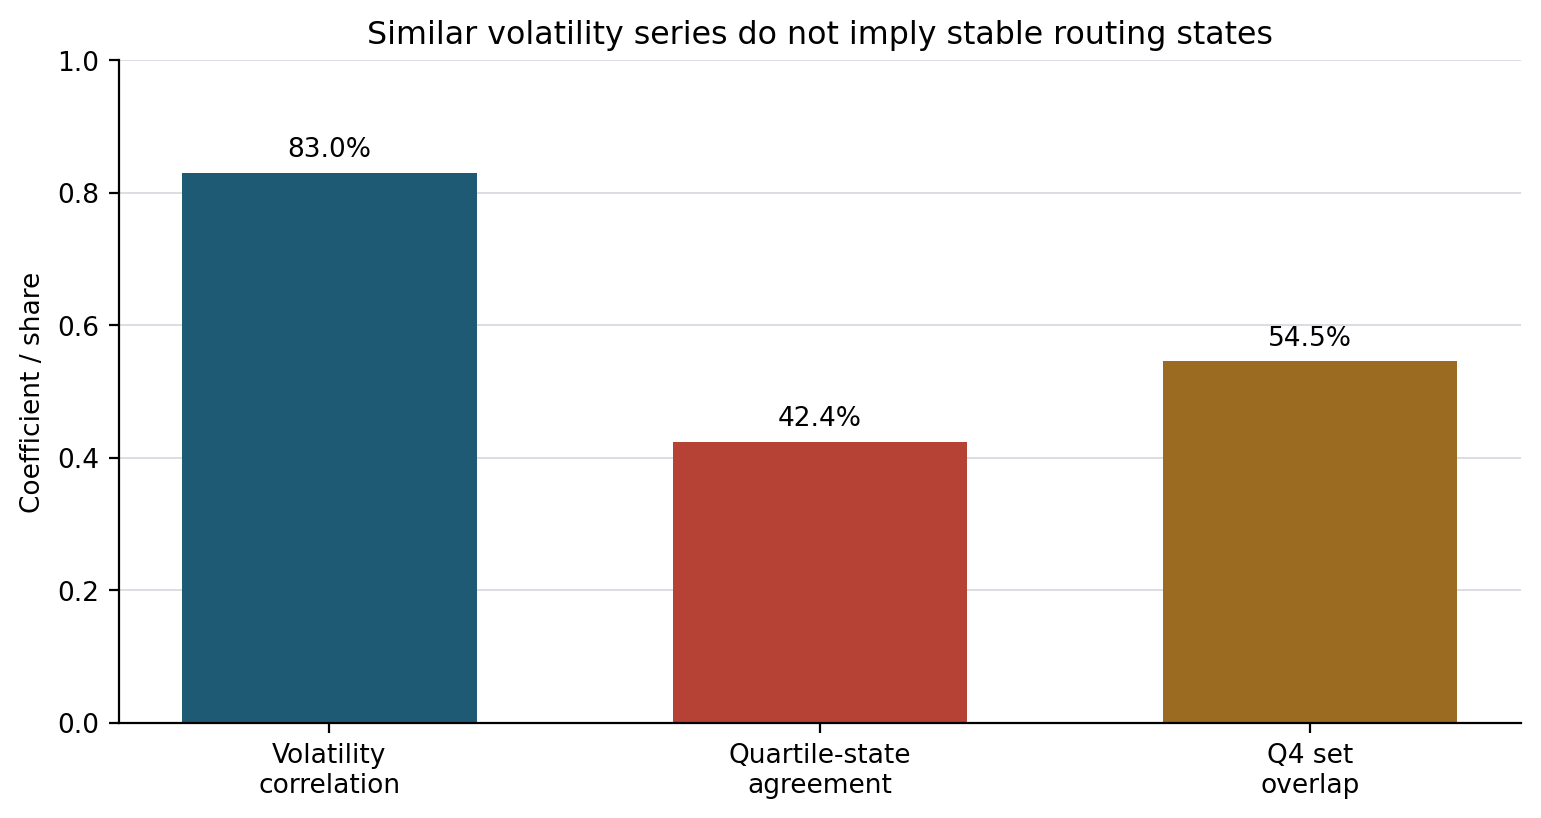
\includegraphics[width=0.78\textwidth]{fig03_public_proxy_stability.png}
\caption{Aggregate agreement between the two pre-specified futures-market volatility
proxies.}
\label{fig:stability}
\end{figure}

This disagreement is not a technical nuisance. Open-interest-notional weighting asks
where outstanding notional activity is concentrated; equal weighting asks what happens
to the typical product. Futures have no theorem that makes either object the unique
``market portfolio.'' A successful router must either survive both or provide an
economic reason why one proxy is causally tied to sleeve failure.

\subsection{High volatility does identify stronger common shocks}

The failure is not explained by Q4 being random. Under the primary proxy, average
pairwise product correlation rises from 0.147 in Q1 to 0.254 in Q4. Average
cross-sectional dispersion rises from 1.21\% to 1.71\%, and directional coherence rises
from 0.300 to 0.376. Q4 therefore represents a more systemic and more heterogeneous
shock environment.

\begin{figure}[H]
\centering
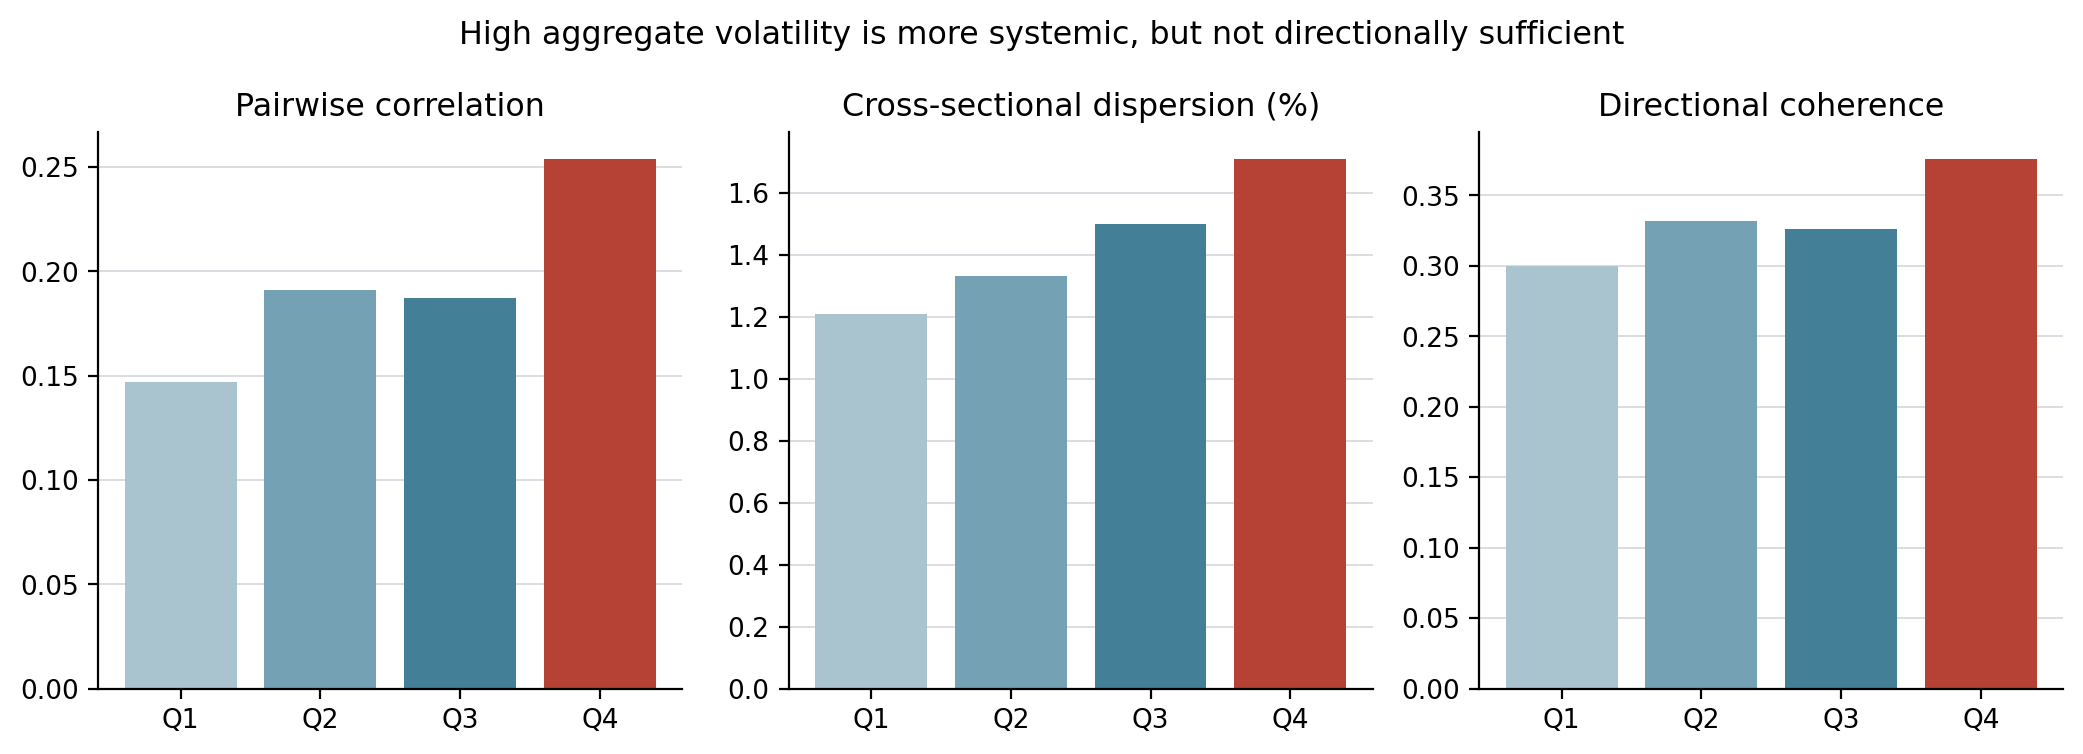
\includegraphics[width=0.96\textwidth]{fig04_public_market_anatomy.png}
\caption{Cross-sectional market anatomy in the primary proxy's signal month.}
\label{fig:anatomy}
\end{figure}

The simultaneous increase in correlation and dispersion is revealing. More products move
in a common direction, while the magnitude of their responses becomes more unequal. This
can arise when a common macro shock is transmitted through products with different
exposures, or when several large sector shocks coincide. Neither case determines whether
the cross-sectional ranking will reverse next month.

\subsection{Intensity is a scalar; strategy state is a vector}

Volatility answers how large price changes are. A momentum--reversal decision additionally
depends on at least four dimensions:

\begin{enumerate}
  \item \textbf{Direction:} a distressed decline followed by rebound versus a directional
  repricing that continues;
  \item \textbf{Source:} demand, supply, inventory, policy, funding, currency, or liquidity;
  \item \textbf{Breadth:} broad participation versus concentration in a subset of large
  products;
  \item \textbf{Stage:} shock initiation, continued absorption, crowded liquidation, or
  exhaustion and repair.
\end{enumerate}

Two months can have the same $\sigma_t$ and differ along every dimension above. The
equity result can be understood as a setting in which high volatility more reliably
coincides with a particular distress-and-rebound vector. The futures cross-section mixes
trend-generating physical shocks with reversal-generating liquidity shocks. A scalar
cannot identify which one is present.

\section{Robustness and Failure Audit}

\subsection{Predefined diagnostic gates}

We distinguish source-direction checks from robust replication. The primary sample can
pass a directional check---reversal loses slightly less than momentum in Q4---while
failing every stability condition needed for a usable router.

\begin{table}[H]
\centering
\caption{Robust replication diagnostics}
\label{tab:gates}
\begin{tabularx}{\textwidth}{YcY}
\toprule
Diagnostic & Passed & Interpretation \\
\midrule
Primary Q4 reversal mean is positive & No & Replacement sleeve still loses in Q4 \\
Primary Q4 reversal wins at least half of months & No & Wins in 4 of 14 months \\
Primary router increment has HAC $t\geq 1$ & No & Increment $t=0.06$ \\
Equal-proxy Q4 reversal exceeds momentum & No & Q4 ranking reverses \\
Equal-proxy router exceeds momentum & No & Router endpoint is lower \\
Positive increment is broad across time & No & One event determines the sign \\
\bottomrule
\end{tabularx}
\end{table}

The failure is overdetermined: it does not rest on one conventional significance cutoff.
It appears in sign stability, win frequency, event influence, market-proxy sensitivity,
and benchmark ranking.

\subsection{Why no percentile search follows}

It would be straightforward to search for a volatility percentile at which the primary
sample looks better. Such a search would answer a different question. The source paper's
75th-percentile rule was the object of replication; the current evidence indicates that
volatility does not impose a stable ordering on the sleeves. Optimizing a boundary on a
non-monotonic and proxy-sensitive relation would primarily fit the locations of a small
number of events.

For the same reason, we do not remove products or sectors based on historical
contribution. Outcome-based universe reduction would change the cross-market replication
into a strategy-selection exercise and understate specification uncertainty.

\subsection{Indicative implementation evidence}

An indicative implementation check applied product-specific fee conventions and uniform
adverse slippage. It did not change the economic ranking between the primary router and
momentum. The difference remained small relative to model and path uncertainty. We do
not report execution parameters or interpret this translation as a fully implementable
portfolio: it excludes integer-lot positioning, capacity, exchange-limit, and margin
models. Detailed execution research is unnecessary until the gross mechanism is stable.

\section{Limitations and Research Implications}

\subsection{What the evidence does not establish}

The sample begins in 2016 and yields 66 evaluable months because five years are consumed
by state formation. Fourteen primary-proxy Q4 observations provide limited power for a
tail-state claim. The study uses daily data and monthly sleeves; it says nothing direct
about minute-level or order-book reversal. It also tests one published momentum window,
one reversal window, one quantile boundary, and two market proxies. Failure to replicate
this rule is not proof that every volatility-aware allocation is ineffective.

Nor does the study show that Chinese futures lack momentum. The frozen momentum sleeve is
positive in the sample. It does not rule out reversal at other horizons or during
particular market events. Finally, the cross-sectional anatomy diagnostics are
descriptive. They show that Q4 is more systemic, but they do not causally identify which
economic shock produced each state.

\subsection{What can be learned from a failed replication}

The failure changes the object of research. The useful question is no longer ``which
volatility percentile maximizes the backtest?'' It is ``which high-volatility states
destroy trends, and which create trends?'' That question is both more economic and more
falsifiable.

A future state model should be low-dimensional and interpretable. It might combine shock
intensity with pre-specified measures of market direction, breadth, and shock stage. Each
additional dimension must first explain the future reversal-minus-momentum spread across
time partitions and reasonable market proxies. Only a mechanism that passes those gates
should be translated into a router and tested on an untouched period.

This sequence matters for inference. Adding indicators until a router improves on the
same 66 months would merely transfer overfitting from a scalar threshold to a state
classifier. Mechanism diagnostics, portfolio selection, and final validation must remain
separate stages.

\subsection{General implication for model transportability}

State variables are not portable solely because their mathematical definitions are
portable. A volatility standard deviation has the same formula in equities and futures,
but its economic content depends on the aggregation object and on which shocks dominate
the market. Cross-market replication should therefore audit three layers:

\begin{enumerate}
  \item \textbf{Measurement invariance:} does the state have a unique or stable market
  definition?
  \item \textbf{Mechanism invariance:} does the state proxy the same economic forces?
  \item \textbf{Decision invariance:} does crossing the state boundary select the same
  return-generating behavior?
\end{enumerate}

The present replication fails all three strongly enough that endpoint outperformance in
one proxy is not persuasive evidence of transportability.

\section{Conclusion}

We replicate a fixed equity volatility-routing method in a broad Chinese futures
cross-section. The primary market proxy produces a superficial echo of the source result:
the router has a slightly higher endpoint than momentum, and one high-volatility event is
successfully hedged by reversal. The broader evidence rejects a stable replication. The
increment is statistically negligible, reversal wins in a minority of Q4 months, the
representative Q4 observation favors momentum, and an equal-product volatility proxy
reverses the key conditional ranking.

At the same time, high volatility is economically meaningful. It identifies months with
higher cross-product correlation, dispersion, and directional coherence. The failure is
therefore not that volatility measures nothing. It is that shock intensity is not a
sufficient statistic for shock type.

This distinction explains why a scalar state can be effective in one asset class and fail
in another without contradiction. In an equity market, high volatility may reliably
proxy a distress, funding, liquidity, and rebound configuration. In a heterogeneous
futures market, high volatility can arise from physical scarcity, policy repricing,
macro risk, or forced trading, with different implications for continuation and reversal.

The appropriate conclusion is narrow: the published volatility-only router does not
robustly transport to this Chinese-futures sample under the pre-specified mapping. The
result does not justify a new optimized percentile. It motivates a more disciplined
research design in which direction, breadth, and stage are treated as explicit hypotheses
and any resulting router is evaluated only after the mechanism is frozen.


\bibliographystyle{apalike}
\bibliography{references}

\clearpage
\appendix
\section{Public Evidence Contract}

\subsection{Sanitization boundary}

The manuscript and all five figures build from a single reviewed JSON file containing
rounded aggregate statistics. The public evidence package excludes source-data files,
contract identifiers, target positions, product- and sector-level PnL attribution,
return time series, event dates, account assumptions, and execution schedules. The
figure builder reads no other research input.

This separation serves two purposes. It prevents accidental disclosure of proprietary
research surfaces, and it makes every public empirical claim auditable against a compact
allowlist. Rounding can create small arithmetic differences between displayed aggregates;
no inference is recomputed from rounded values.

\subsection{Methodology lock}

Before the replication returns were inspected, the following objects were fixed:

\begin{itemize}
  \item causal daily main-contract construction and same-contract returns;
  \item 11-month momentum formation with a one-month skip;
  \item one-month reversal formation;
  \item equal-weight top and bottom 10\% portfolio legs;
  \item a 60-month volatility distribution and fixed Q4 switch;
  \item one-month signal-to-holding lag;
  \item primary lagged open-interest-notional and equal-product market proxies;
  \item prohibition of threshold, sector, product, and universe selection.
\end{itemize}

\subsection{Reproduction of public figures}

The public figures can be rebuilt with the standalone script described in the project
README. The boundary test verifies that the public tree contains no private research
paths, contract-level files, source hashes, or disallowed execution fields, and that the
figure script reads only the aggregate evidence JSON.

\section{Additional Aggregate Tables}

\begin{table}[H]
\centering
\caption{Conditional mean monthly gross returns (percent)}
\begin{tabular}{llrrr}
\toprule
Proxy & State & Months & Momentum & Reversal \\
\midrule
OI-notional & Q1 & 21 & 0.66 & $-0.12$ \\
OI-notional & Q2 & 17 & $-0.92$ & 2.86 \\
OI-notional & Q3 & 14 & 6.04 & $-3.89$ \\
OI-notional & Q4 & 14 & $-0.71$ & $-0.54$ \\
\midrule
Equal product & Q1 & 12 & 5.20 & $-1.97$ \\
Equal product & Q2 & 15 & $-1.07$ & $-1.05$ \\
Equal product & Q3 & 19 & $-1.14$ & 0.29 \\
Equal product & Q4 & 20 & 2.40 & 0.90 \\
\bottomrule
\end{tabular}
\end{table}

\begin{table}[H]
\centering
\caption{Primary-proxy cross-sectional anatomy by signal state}
\begin{tabular}{lrrr}
\toprule
State & Pairwise correlation & Dispersion & Directional coherence \\
\midrule
Q1 & 0.147 & 1.21\% & 0.300 \\
Q2 & 0.191 & 1.33\% & 0.332 \\
Q3 & 0.187 & 1.50\% & 0.326 \\
Q4 & 0.254 & 1.71\% & 0.376 \\
\bottomrule
\end{tabular}
\end{table}


\end{document}
